\documentclass[a4paper]{article}

\usepackage[pdftex,
  hidelinks,
  pdfauthor={Dexter Chua},
  pdfsubject={Cambridge Maths Notes: Part II - Logic and Set Theory},
  pdftitle={Part IB - Logic and Set Theory},
pdfkeywords={Cambridge Mathematics Maths Math II Lent Logic and Set Theory}]{hyperref}

\title{Part II - Logic and Set Theory}
\author{Lectured by I. B. Leader}
\date{Lent 2015}

% Imports
\ifx \nextra \undefined
  \usepackage[pdftex,
    hidelinks,
    pdfauthor={Dexter Chua},
    pdfsubject={Cambridge Maths Notes: Part \npart\ - \ncourse},
    pdftitle={Part \npart\ - \ncourse},
  pdfkeywords={Cambridge Mathematics Maths Math \npart\ \nterm\ \nyear\ \ncourse}]{hyperref}
  \title{Part \npart\ - \ncourse}
\else
  \usepackage[pdftex,
    hidelinks,
    pdfauthor={Dexter Chua},
    pdfsubject={Cambridge Maths Notes: Part \npart\ - \ncourse\ (\nextra)},
    pdftitle={Part \npart\ - \ncourse\ (\nextra)},
  pdfkeywords={Cambridge Mathematics Maths Math \npart\ \nterm\ \nyear\ \ncourse\ \nextra}]{hyperref}

  \title{Part \npart\ - \ncourse \\ {\Large \nextra}}
\fi

\author{Lectured by \nlecturer \\\small Notes taken by Dexter Chua}
\date{\nterm\ \nyear}

\usepackage{alltt}
\usepackage{amsfonts}
\usepackage{amsmath}
\usepackage{amssymb}
\usepackage{amsthm}
\usepackage{booktabs}
\usepackage{caption}
\usepackage{enumitem}
\usepackage{fancyhdr}
\usepackage{graphicx}
\usepackage{mathtools}
\usepackage{microtype}
\usepackage{multirow}
\usepackage{pdflscape}
\usepackage{pgfplots}
\usepackage{siunitx}
\usepackage{tabularx}
\usepackage{tikz}
\usepackage{tkz-euclide}
\usepackage[normalem]{ulem}
\usepackage[all]{xy}

\pgfplotsset{compat=1.12}

\pagestyle{fancyplain}
\lhead{\emph{\nouppercase{\leftmark}}}
\ifx \nextra \undefined
  \rhead{
    \ifnum\thepage=1
    \else
      \npart\ \ncourse
    \fi}
\else
  \rhead{
    \ifnum\thepage=1
    \else
      \npart\ \ncourse\ (\nextra)
    \fi}
\fi
\usetikzlibrary{arrows}
\usetikzlibrary{decorations.markings}
\usetikzlibrary{decorations.pathmorphing}
\usetikzlibrary{positioning}
\usetikzlibrary{fadings}
\usetikzlibrary{intersections}
\usetikzlibrary{cd}

\newcommand*{\Cdot}{\raisebox{-0.25ex}{\scalebox{1.5}{$\cdot$}}}
\newcommand {\pd}[2][ ]{
  \ifx #1 { }
    \frac{\partial}{\partial #2}
  \else
    \frac{\partial^{#1}}{\partial #2^{#1}}
  \fi
}

% Theorems
\theoremstyle{definition}
\newtheorem*{aim}{Aim}
\newtheorem*{axiom}{Axiom}
\newtheorem*{claim}{Claim}
\newtheorem*{cor}{Corollary}
\newtheorem*{defi}{Definition}
\newtheorem*{eg}{Example}
\newtheorem*{fact}{Fact}
\newtheorem*{law}{Law}
\newtheorem*{lemma}{Lemma}
\newtheorem*{notation}{Notation}
\newtheorem*{prop}{Proposition}
\newtheorem*{thm}{Theorem}

\renewcommand{\labelitemi}{--}
\renewcommand{\labelitemii}{$\circ$}
\renewcommand{\labelenumi}{(\roman{*})}

\let\stdsection\section
\renewcommand\section{\newpage\stdsection}

% Strike through
\def\st{\bgroup \ULdepth=-.55ex \ULset}

% Maths symbols
\newcommand{\bra}{\langle}
\newcommand{\ket}{\rangle}

\newcommand{\N}{\mathbb{N}}
\newcommand{\Z}{\mathbb{Z}}
\newcommand{\Q}{\mathbb{Q}}
\renewcommand{\H}{\mathbb{H}}
\newcommand{\R}{\mathbb{R}}
\newcommand{\C}{\mathbb{C}}
\newcommand{\Prob}{\mathbb{P}}
\renewcommand{\P}{\mathbb{P}}
\newcommand{\E}{\mathbb{E}}
\newcommand{\F}{\mathbb{F}}
\newcommand{\cU}{\mathcal{U}}
\newcommand{\RP}{\mathbb{RP}}
\newcommand{\CP}{\mathbb{CP}}

\newcommand{\ph}{\,\cdot\,}

\DeclareMathOperator{\sech}{sech}
\DeclareMathOperator{\cosech}{cosech}
\DeclareMathOperator{\cosec}{cosec}

\DeclareMathOperator{\covol}{covol}
\DeclareMathOperator{\vol}{vol}

\let\Im\relax
\let\Re\relax
\DeclareMathOperator{\Im}{Im}
\DeclareMathOperator{\Re}{Re}
\DeclareMathOperator{\im}{im}
\DeclareMathOperator{\image}{image}
\DeclareMathOperator{\Ann}{Ann}

\DeclareMathOperator*{\res}{res}
\DeclareMathOperator{\Res}{Res}
\DeclareMathOperator{\Ind}{Ind}

\DeclareMathOperator{\tr}{tr}
\DeclareMathOperator{\diag}{diag}
\DeclareMathOperator{\rank}{rank}
\DeclareMathOperator{\card}{card}
\DeclareMathOperator{\spn}{span}
\DeclareMathOperator{\adj}{adj}

\DeclareMathOperator{\erf}{erf}
\DeclareMathOperator{\erfc}{erfc}

\DeclareMathOperator{\ord}{ord}
\DeclareMathOperator{\Sym}{Sym}

\DeclareMathOperator{\sgn}{sgn}
\DeclareMathOperator{\orb}{orb}
\DeclareMathOperator{\stab}{stab}
\DeclareMathOperator{\ccl}{ccl}

\DeclareMathOperator{\lcm}{lcm}
\DeclareMathOperator{\hcf}{hcf}

\DeclareMathOperator{\Int}{Int}
\DeclareMathOperator{\id}{id}

\DeclareMathOperator{\betaD}{beta}
\DeclareMathOperator{\gammaD}{gamma}
\DeclareMathOperator{\Poisson}{Poisson}
\DeclareMathOperator{\binomial}{binomial}
\DeclareMathOperator{\multinomial}{multinomial}
\DeclareMathOperator{\Bernoulli}{Bernoulli}
\DeclareMathOperator{\like}{like}

\DeclareMathOperator{\var}{var}
\DeclareMathOperator{\cov}{cov}
\DeclareMathOperator{\bias}{bias}
\DeclareMathOperator{\mse}{mse}
\DeclareMathOperator{\corr}{corr}

\DeclareMathOperator{\otp}{otp}
\DeclareMathOperator{\dom}{dom}

\DeclareMathOperator{\Root}{Root}
\DeclareMathOperator{\supp}{supp}
\DeclareMathOperator{\rel}{rel}
\DeclareMathOperator{\Hom}{Hom}
\DeclareMathOperator{\Aut}{Aut}
\DeclareMathOperator{\Gal}{Gal}
\DeclareMathOperator{\Mat}{Mat}
\DeclareMathOperator{\End}{End}
\DeclareMathOperator{\Char}{char}
\DeclareMathOperator{\ev}{ev}
\DeclareMathOperator{\St}{St}
\DeclareMathOperator{\Lk}{Lk}
\DeclareMathOperator{\disc}{disc}
\DeclareMathOperator{\Isom}{Isom}
\DeclareMathOperator{\length}{length}
\DeclareMathOperator{\energy}{energy}
\DeclareMathOperator{\area}{area}
\DeclareMathOperator{\Syl}{Syl}
\DeclareMathOperator{\cl}{cl}
\DeclareMathOperator{\fix}{fix}

\newcommand{\GL}{\mathrm{GL}}
\newcommand{\SL}{\mathrm{SL}}
\newcommand{\PGL}{\mathrm{PGL}}
\newcommand{\PSL}{\mathrm{PSL}}
\newcommand{\PSU}{\mathrm{PSU}}
\newcommand{\Or}{\mathrm{O}}
\newcommand{\SO}{\mathrm{SO}}
\newcommand{\U}{\mathrm{U}}
\newcommand{\SU}{\mathrm{SU}}

\renewcommand{\d}{\mathrm{d}}
\newcommand{\D}{\mathrm{D}}

\tikzset{->/.style = {decoration={markings,
                                  mark=at position 1 with {\arrow[scale=2]{latex'}}},
                      postaction={decorate}}}
\tikzset{<-/.style = {decoration={markings,
                                  mark=at position 0 with {\arrowreversed[scale=2]{latex'}}},
                      postaction={decorate}}}
\tikzset{<->/.style = {decoration={markings,
                                   mark=at position 0 with {\arrowreversed[scale=2]{latex'}},
                                   mark=at position 1 with {\arrow[scale=2]{latex'}}},
                       postaction={decorate}}}
\tikzset{->-/.style = {decoration={markings,
                                   mark=at position #1 with {\arrow[scale=2]{latex'}}},
                       postaction={decorate}}}
\tikzset{-<-/.style = {decoration={markings,
                                   mark=at position #1 with {\arrowreversed[scale=2]{latex'}}},
                       postaction={decorate}}}

\tikzset{circ/.style = {fill, circle, inner sep = 0, minimum size = 3}}
\tikzset{mstate/.style={circle, draw, blue, text=black, minimum width=0.7cm}}

\definecolor{mblue}{rgb}{0.2, 0.3, 0.8}
\definecolor{morange}{rgb}{1, 0.5, 0}
\definecolor{mgreen}{rgb}{0.1, 0.4, 0.2}
\definecolor{mred}{rgb}{0.5, 0, 0}

\def\drawcirculararc(#1,#2)(#3,#4)(#5,#6){%
    \pgfmathsetmacro\cA{(#1*#1+#2*#2-#3*#3-#4*#4)/2}%
    \pgfmathsetmacro\cB{(#1*#1+#2*#2-#5*#5-#6*#6)/2}%
    \pgfmathsetmacro\cy{(\cB*(#1-#3)-\cA*(#1-#5))/%
                        ((#2-#6)*(#1-#3)-(#2-#4)*(#1-#5))}%
    \pgfmathsetmacro\cx{(\cA-\cy*(#2-#4))/(#1-#3)}%
    \pgfmathsetmacro\cr{sqrt((#1-\cx)*(#1-\cx)+(#2-\cy)*(#2-\cy))}%
    \pgfmathsetmacro\cA{atan2(#2-\cy,#1-\cx)}%
    \pgfmathsetmacro\cB{atan2(#6-\cy,#5-\cx)}%
    \pgfmathparse{\cB<\cA}%
    \ifnum\pgfmathresult=1
        \pgfmathsetmacro\cB{\cB+360}%
    \fi
    \draw (#1,#2) arc (\cA:\cB:\cr);%
}
\newcommand\getCoord[3]{\newdimen{#1}\newdimen{#2}\pgfextractx{#1}{\pgfpointanchor{#3}{center}}\pgfextracty{#2}{\pgfpointanchor{#3}{center}}}

\def\Xint#1{\mathchoice
   {\XXint\displaystyle\textstyle{#1}}%
   {\XXint\textstyle\scriptstyle{#1}}%
   {\XXint\scriptstyle\scriptscriptstyle{#1}}%
   {\XXint\scriptscriptstyle\scriptscriptstyle{#1}}%
   \!\int}
\def\XXint#1#2#3{{\setbox0=\hbox{$#1{#2#3}{\int}$}
     \vcenter{\hbox{$#2#3$}}\kern-.5\wd0}}
\def\ddashint{\Xint=}
\def\dashint{\Xint-}


\begin{document}
\maketitle
{\small
  \noindent\textbf{Ordinals and cardinals}\\
  Well-orderings and order-types. Examples of countable ordinals. Uncountable ordinals and Hartogs' lemma. Induction and recursion for ordinals. Ordinal arithmetic. Cardinals; the hierarchy of alephs. Cardinal arithmetic.\hspace*{\fill} [5]

  \vspace{10pt}
  \noindent\textbf{Posets and Zorn's lemma}\\
  Partially ordered sets; Hasse diagrams, chains, maximal elements. Lattices and Boolean algebras. Complete and chain-complete posets; fixed-point theorems. The axiom of choice and Zorn's lemma. Applications of Zorn's lemma in mathematics. The well-ordering principle.\hspace*{\fill} [5]

  \vspace{10pt}
  \noindent\textbf{Propositional logic}\\
  The propositional calculus. Semantic and syntactic entailment. The deduction and completeness theorems. Applications: compactness and decidability.\hspace*{\fill} [3]

  \vspace{10pt}
  \noindent\textbf{Predicate logic}\\
  The predicate calculus with equality. Examples of first-order languages and theories. Statement of the completeness theorem; *sketch of proof*. The compactness theorem and the Lowenheim-Skolem theorems. Limitations of first-order logic. Model theory.\hspace*{\fill} [5]

  \vspace{10pt}
  \noindent\textbf{Set theory}\\ Set theory as a first-order theory; the axioms of ZF set theory. Transitive closures, epsilon-induction and epsilon-recursion. Well-founded relations. Mostowski's collapsing theorem. The rank function and the von Neumann hierarchy.\hspace*{\fill} [5]
  
  \vspace{10pt}
  \noindent\textbf{Consistency}\\
  *Problems of consistency and independence*\hspace*{\fill} [1]}

\tableofcontents

\section{Propositional calculus}
\begin{defi}[Propositions]
  Let $P$ be a set of \emph{primitive propositions}. These are a bunch of (meaningless) symbols, that are usually interpreted to take a truth value. Usually, any symbol (composed of alphabets and subscripts) is in the set of primitive propositions.

  The set of \emph{propositions}, written as $L$ or $L(P)$, is defined inductively by
  \begin{enumerate}
    \item If $p\in P$, then $p\in L$.
    \item $\bot\in L$, where $\bot$ is ``false'' (also a meaningless symbol).
    \item If $p, q\in L$, then $p\Rightarrow q)\in L$.
  \end{enumerate}
\end{defi}

\begin{eg}
  $p\Rightarrow q$, $p\Rightarrow \bot$, $((p\Rightarrow q)\Rightarrow (p\Rightarrow r))$ are propositions.
\end{eg}

To define $L$ formally, we let $L_1 = \{\bot\}\cup P$, and for $n\geq 1$, $L_{n + 1} = L_n\cup \{(p\Rightarrow q): p, q\in L_n\}$. Then set $L = L_1\cup L_2\cup \cdots$.

In formal language terms, $L$ is the set of finite strings of symbols from the alphabet $\bot$, $\bot$, $\Rightarrow $, $($, $)$, $p_1$, $p_2, \cdots$ that satisfies some formal grammar rule (eg. brackets have to match).

We define the following abbreviations:
\begin{defi}[Logical symbols]\leavevmode
  \begin{center}
    \begin{tabular}[]{cccc}
      $\neg p$ & (``not $p$'') & is an abbreviation for & $(p\Rightarrow \bot)$\\
      $p\wedge q$ & (``$p$ and $q$'') & is an abbreviation for & $\neg(p\Rightarrow (\neg q))$\\
      $p\vee q$ & (``$p$ or $q$'') & is an abbreviation for & $(\neg p)\Rightarrow q$
    \end{tabular}
  \end{center}
\end{defi}
\subsection{Semantic implication}
\begin{defi}[Valuation]
  A \emph{valuation} on $L$ is a function $v: L\to \{0, 1\}$ such that:
  \begin{itemize}
  \item $v(\bot) = 0$,
  \item $v(p\Rightarrow q) = \begin{cases} 0 & \text{if }v(p) = 1, v(q) = 0,\\1 & \text{otherwise}\end{cases}$
  \end{itemize}
  We interpret $v(p)$ to be the truth value of $p$, with 0 denoting ``false'' and 1 denoting ``true''.

  Note that we do not impose any restriction of $v(p)$ when $p$ is a primitive proposition (that is not $\bot$).
\end{defi}

We can also give $\{0, 1\}$ a binary operation $\Rightarrow$ by
\[
  a\Rightarrow b = \begin{cases}
    0 & \text{if }a = 1, b = 0\\
    1 & \text{otherwise}
  \end{cases}
\]
with a constant $\bot = 0$. Then a valuation $v: K\to \{0, 1\}$ is simply a homomorphism between the two structures that preserve $\bot$ and $\Rightarrow $.

\begin{prop}\leavevmode
  \begin{enumerate}
    \item If $v$ and $v'$ are valuations with $v(p) = v'(p)$ for all $p\in P$, then $v = v'$.
    \item For any function $W: P \to \{0, 1\}$, there is a valuation $v$ such that $v(p) = w(p)$ for all $p\in L$, ie. we can extend $w$ to a full valuation.
  \end{enumerate}
  This means ``A valuation is determined by its values on $P$, and any values will do''.
\end{prop}

\begin{proof}
  \begin{enumerate}
    \item Recall that $L$ is defined inductively. We are given that $v(p) = v'(p)$ on $L_1$. Then for all $p\in L_2$, $p$ must be in the form $q\Rightarrow r$ for $q, r\in L_1$. Then $v(q\Rightarrow r) = v(p\Rightarrow q)$ since the value of $v$ is uniquely determined by the definition. So for all $p\in L_2$, $v(p) = v'(p)$.

      Continue inductively to show that $v(p) = v'(p)$ for all $p\in L_n$ for any $n$.
    
    \item Set $v$ to agree with $w$ for all $p\in P$, and set $v(\bot) = 0$. Then define $v$ on $L_n$ inductively according to the definition.
  \end{enumerate}
\end{proof}

\begin{eg}
  Suppose $v$ is a valuation with $v(p) = v(q) = 1$, $v(r) = 0$. Then
  \[
    v((p\Rightarrow q)\Rightarrow r) = 0.
  \]
\end{eg}

\begin{defi}[Tautology]
  $t$ is a \emph{tautology}, written as $\models t$, if $v(t) = 1$. 
\end{defi}

\begin{eg}
  \begin{enumerate}
    \item $p\Rightarrow (q\Rightarrow p)$ ``A true statement is implied by anything''.\vspace{5pt}\\
      \begin{tabular}[]{cccc}
        $v(p)$ & $v(q)$ & $v(q\Rightarrow p)$ & $v(p\Rightarrow (q\Rightarrow p))$\\
        1 & 1 & 1 & 1\\
        1 & 0 & 1 & 1\\
        0 & 1 & 0 & 1\\
        0 & 0 & 1 & 1
      \end{tabular}
    \item $(\neg \neg p)\Rightarrow p$. Recall that $\neg\neg p$ is defined as $((p\Rightarrow \bot)\Rightarrow \bot)$.\vspace{5pt}\\
    \begin{tabular}{cccc}
      $v(p)$ & $v(p\Rightarrow \bot)$ & $v((p\Rightarrow \bot)\Rightarrow \bot)$ & $v(((p\Rightarrow \bot)\Rightarrow \bot)\Rightarrow p)$\\
      1 & 0 & 1 & 1\\
      0 & 1 & 0 & 1
    \end{tabular}
  \item $(p\Rightarrow (q\Rightarrow r))\Rightarrow ((p\Rightarrow q)\Rightarrow (p\Rightarrow r))$.

    Instead of creating a truth table, which would be horribly long, we show this by reasoning: Suppose it is not a tautology. So there is a $v$ such that $v(p\Rightarrow q\Rightarrow r)) = 1$ and $v((p\Rightarrow q)\Rightarrow (p\Rightarrow r)) =0 $. For the second equality to hold, we must have $v(p\Rightarrow q) = 1$ and $v(p\Rightarrow r) = 0$. So $v(p) = 1, v(r) = 0, v(q) = 1$. But then $v(p\Rightarrow q) = 0$. 
  \end{enumerate}
\end{eg}

\begin{defi}[Semantic entailment]
  For $S\subseteq L$, $t\in L$, we say $S$ \emph{entails} $t$, $S$ \emph{semantically implies t} or $S\models t$ if, for any $v$ such that $v(s) = 1$ for all $s\in S$, $v(t) = 1$.

  ``Whenever all of $S$ is true, $t$ is true as well.''
\end{defi}

\begin{eg}
  $\{p\Rightarrow q, q\Rightarrow r\}\models (p\Rightarrow r).$

  We want to show that for any valuation $v$ with $v(p\Rightarrow q) = v(q\Rightarrow r) = 1$, we have $v(p\Rightarrow r) = 1$. We prove the contrapositive.

  If $v(p\Rightarrow r) = 0$, then $v(p) = 1$ and $v(r) = 0$. If $v(q) = 0$, then $v(p\Rightarrow q) = 0$. If $v(q) = 1$, then $v(q\Rightarrow r) = 0$. So $v(p\Rightarrow r) = 0$ only if one of $v(p\Rightarrow q)$ or $v(q\Rightarrow r)$ is zero. 
\end{eg}
\begin{defi}[Truth and model]
  If $v(t) = 1$, then we say that $t$ is \emph{true} in $v$, or $v$ is a \emph{model} of $t$. For $S\subseteq L$, a valuation $v$ is a \emph{model} of $S$ if $v(s) = 1$. Then $\models t$ means $\emptyset \models t$. 
\end{defi}
\subsection{Syntactic implication}
While semantic implication captures the idea of truthfulness, syntactic implication captures the idea of proofs. To do so, we need to have axioms and deduction rules.

Our system of deduction composes of the following axioms:
\begin{enumerate}
  \item $p\Rightarrow(q\Rightarrow p)$
  \item $[p\Rightarrow(q\Rightarrow r)]\Rightarrow[(p\Rightarrow q)\Rightarrow(p \Rightarrow r)]$
  \item $(\neg\neg p)\Rightarrow p$
\end{enumerate}
and the deduction rule of \emph{modus ponens}: from $p$ and $p\Rightarrow q$, we can deduce $q$.

Note that every axiom is a tautology. 

\begin{defi}[Proof and syntactic entailment]
  For any $S\subseteq L$, a \emph{proof} of $t$ from $S$ is a finite sequence $t_1, t_2, \cdots t_n$ of propositions, with $t_n = t$, such that each $t_i$ is one of the following:
\begin{enumerate}
  \item An axiom
  \item A member of $S$
  \item A proposition $t_i$ such that there exist $j, k < i$ with $t_j = (t_k\Rightarrow t_i)$.
\end{enumerate}
If there is a proof of $t$ from $S$, we say that $S$ \emph{proves} or \emph{syntactically entails} $t$, written $S\vdash t$.

If $\emptyset \vdash t$, say $t$ is a \emph{theorem} and write $\vdash t$.

In a proof of $t$ from $S$, $t$ is the \emph{conclusion} and $S$ is the set of \emph{hypothesis} or \emph{premises}.


\end{defi}
\begin{eg}
  $\{p\Rightarrow q, q\Rightarrow r\} \vdash p\Rightarrow r$

  ``Go for $(p\Rightarrow  q)\Rightarrow  (p\Rightarrow  r)$ via Axiom 2.
  \begin{enumerate}[label=\arabic{*}.]
    \item $[p\Rightarrow (q\Rightarrow r)]\Rightarrow [(p\Rightarrow q) \Rightarrow (p\Rightarrow r)]$ \hfill Axiom 2
    \item $q\Rightarrow r$ \hfill Hypothesis
    \item $(q\Rightarrow r)\Rightarrow [q\Rightarrow (q\Rightarrow r)]$\hfill Axiom 1
    \item $p\Rightarrow (q\Rightarrow r)$ \hfill MP on 2,3
    \item $(p\Rightarrow q)\Rightarrow (p\Rightarrow r)$\hfill MP on 1, 4
    \item $p\Rightarrow q$\hfill Hypothesis
    \item $p\Rightarrow r$\hfill MP on 5, 6
  \end{enumerate}
\end{eg}

\begin{eg}
  $\vdash (p\Rightarrow p)$

  ``Go for $[p\Rightarrow (p\Rightarrow p)]\Rightarrow (p\Rightarrow p)$''
  \begin{enumerate}[label=\arabic{*}.]
    \item $[p\Rightarrow ((p\Rightarrow p)\Rightarrow p)]\Rightarrow [(p\Rightarrow (p\Rightarrow p))\Rightarrow (p\Rightarrow p)]$ \hfill Axiom 2
    \item $p\Rightarrow ( (p\Rightarrow p)\Rightarrow p)$\hfill Axiom 1
    \item $[p\Rightarrow (p\Rightarrow p)]\Rightarrow (p\Rightarrow p)$ \hfill MP on 1, 2
    \item $p\Rightarrow (p\Rightarrow p)$\hfill Axiom 1
    \item $p\Rightarrow p$ \hfill MP on 3, 4
  \end{enumerate}
\end{eg}

This seems like a really tedious way to prove things. We now prove that the \emph{deduction theorem}, that can usually help to prove $S\vdash t$.

\begin{prop}[Deduction theorem]
  Let $S\subset L$ and $p, q\in L$. Then $S\vdash (p\Rightarrow q)$ if and only if $S\cup {p} \vdash q$.\\

  ``$\vdash$ behaves like the connective $\Rightarrow $ in the language''
\end{prop}

\begin{proof}
  ($\Rightarrow $) Given a proof of $p\Rightarrow q$ from $S$, append the lines
  \begin{itemize}
    \item $p$\hfill Hypothesis
    \item $q$\hfill $MP$
  \end{itemize}
  to obtain a proof of $q$ from $S\cup \{q\}$.

  ($\Leftarrow$) Let $t_1, t_2, \cdots, t_n = q$ be a proof of $q$ from $S\cup \{p\}$. We'll show that $S\vdash p\Rightarrow t_i$ for all $i$.

  We consider different possibilities of $t_i$:
  \begin{itemize}
    \item $t_i$ is an axiom: Write down
      \begin{itemize}
        \item $t_i\Rightarrow (p\Rightarrow t_i)$\hfill (Axiom 1)
        \item $t_i$\hfill Axiom
        \item $p\Rightarrow t_i$ \hfill MP
      \end{itemize}
    \item $t_i\in S$: Write down
      \begin{itemize}
        \item $t_i\Rightarrow (p\Rightarrow t_i)$\hfill (Axiom 1)
        \item $t_i$\hfill Hypothesis
        \item $p\Rightarrow t_i$ \hfill MP
      \end{itemize}
      To get $S\models (p\Rightarrow t_i)$
    \item $t_i = p$: Write down our proof of $p\Rightarrow p$ from our example above.
    \item $t_i$ is obtained by MP: we have some $j, k< i$ such that $t_k = (t_k\Rightarrow t_i)$. We can assume that $S\vdash (p\Rightarrow t_j)$ and $S\vdash (p\Rightarrow t_k)$ by induction on $i$. Now we can write down
      \begin{itemize}
        \item $[p\Rightarrow (t_j\Rightarrow t_i)]\Rightarrow [(p\Rightarrow t_j)\Rightarrow (p\Rightarrow t_i)]$\hfill Axiom 2
        \item $p\Rightarrow (t_j\Rightarrow t_i)$\hfill Known already
        \item $(p\Rightarrow t_j)\Rightarrow (p\Rightarrow t_i)$\hfill MP
        \item $p\Rightarrow t_j$\hfill Known already
        \item $p\Rightarrow t_i$\hfill MP
      \end{itemize}
      to get $S\models (p\Rightarrow t_i)$. 
  \end{itemize}
  This is why Axiom 2 is as it is - it enables us to prove the deduction theorem. 
\end{proof}

\begin{eg}
  We want to show $\{p\Rightarrow  q, q\Rightarrow r\} \vdash (p\Rightarrow r)$. By the deduction theorem, it is enough to show that $\{p\Rightarrow q, q\Rightarrow  r, p\}\vdash r$, which is trivial by applying MP twice. 
\end{eg}

Now we have two notions: $\models$ and $\vdash$. How are they related? We want to show that they are equal: if something is true, we can prove it; if we can prove something, it must be true.

\noindent\textbf{Aim.} Show that $S\vdash t$ if and only if $S\models t$.
This is the \emph{completeness theorem}, made up of two directions:
\begin{enumerate}
  \item Soundness: If $S\vdash t$, then $S\models t$. ``Our axioms aren't absurd''
  \item Adequacy: If $S\models t$, $S\vdash t$.  ``Our axioms are strong enough to be able to deduce, from $S$, \emph{all} semantic consequences of $S$.''
\end{enumerate}

\begin{prop}[Soundness theorem]
  If $S\vdash t$, then $S\models t$.
\end{prop}

\begin{proof}
  Given valuation $v$ with $v(s) = 1$ for all $s\in S$, we need to show that $v(t) = 1$. But $v(p) = 1$ for all axioms $p$, and $v(p) = 1$ for all $p\in S$, and if $v(p) = 1$ and $v(p\Rightarrow q) = 1$, then $v(q) = 1$. Hence each line $t_i$ in a proof $t_1, \cdots, t_n$ of from $S$ has $v(t_i) = 1$. 
\end{proof}
This works because we know that all axioms of tautologies.

We first prove a special case of adequacy:
\begin{defi}[Consistent]
  $S$ is \emph{inconsistent} if $S\vdash \bot$. $S$ is \emph{consistent} if it is not inconsistent.
\end{defi}

We prove the following statement:
\begin{thm}[Model existence theorem]
  If $S\models \bot$, then $S\vdash \bot$. ie., if $S$ has no model, then $S$ is consistent. ie. If $S$ is consistent, then $S$ has a model.

  \note Some books call this the ``completeness theorem'', because the rest of the completeness theorem follows trivially from this. 
\end{thm}

In fact, this would imply adequacy. Indeed if $S\models t$, then  $S\cup \{\neg t\}\models \bot$. Hence $S\cup \{\neg t\}\vdash \bot$ by our special case. So $S\vdash \neg \neg t$ by the deduction theorem. But $\vdash (\neg\neg t)\Rightarrow t$ by Axiom 3. So $S\vdash t$.

\begin{proof}
  The idea is that we'd like to define $v: L \to \{0, 1\}$ by
  \[
    p\mapsto
    \begin{cases}
      1 & \text{if } p\in S\\
      0 & \text{if } p\in S
    \end{cases}
  \]
  However, this is obviously going to fail, because we might have implications of $S$ that are not in $S$, ie. $S$ is not \emph{deductively closed} (deductively closed means $S\vdash p$ implies $p\in S$). Yet this is not a serious problem - we take the deductive closure first.

  But there is a more serious problem. There might be a $p$ with $S\not\vdash p$ and $S\not\vdash \neg p$. This is the case if $p$ never appears in $S$. We'll try to extend $S$ to ``swallow up'' half of $L$. ie. we give $p$ an arbitrary truth value, without making $S$ inconsistent. The meat of this proof is then to see that we can ``swallow up'' propositions consistently.

  We first try to swallow up one proposition only.
  
  \noindent\textbf{Claim.} For consistent $S\subset L$ and $p\in L$, we have $S\cup \{p\}$ or $S\cup \{\neg p\}$ consistent.

  Suppose instead that $S\cup \{p\} \vdash \bot$ and $S\cup \{\neg p\}\vdash \bot$.Then by the deduction theorem, $S\vdash p$ and $S\vdash \neg p$. So $S\vdash \bot$.

  As a general rule of mathematics, after doing it for one thing, we do it for infinitely many things.

  Now we suppose $L$ is countable. So we can list $L$ as $\{t_1, t_2, \cdots\}$.

  Let $S_0 = S$. Then let $S_1 = S\cup \{t_1\}$ or $S\cup \{\neg t_1\}$ such that $S_1$ is consistent, and let $S_2 = S_1 \cup \{t_2\}$ or $S_1\cup \{\neg t_2\}$ such that $S_2$ is consistent. Continue inductively.

  Set $\bar{S} = S_0\cup S_1\cup S_2\cdot$. Then $p\in \bar{S}$ or $\neg p\in \bar{S}$ for each $p\in l$ by construction. Also $\bar S$ is consistent (If $\bar S\vdash \bot$, then some $S_n\vdash \bot$ since proofs are finite, but all $S_n$ are consistent). Finally, we check that $\bar S$ is deductively closed, since if $\bar S\models p$, and $p\not\in \bar S$, then $\neg p\not\in \bar S$. Then $\bar S$ would be inconsistent.

  Define $v: L\to \{0, 1\}$ by
  \[
    p \mapsto
    \begin{cases}
      1 & \text{if }p\in \bar S\\
      0 & \text{if not}
    \end{cases}.
  \]
  We claim this is a valuation:

  $v(\bot) = 0$ as $\bot \not\in \bar S$ (since $\bar S$ is consistent).

  For $p\Rightarrow q$,
  \begin{enumerate}
    \item If $v(p) = 1, v(q) = 0$, we have $p\in \bar S$, $q\not\in \bar S$. We want to show $p\Rightarrow q\not\in \bar S$. But if $p\Rightarrow q\in \bar S$, then $\bar S \vdash q$ by MP. Hence $q\in \bar S$ since $\bar S$ is deductively closed.
    \item If $v(q) = 1$, then $q\in \bar S$. We want $p\Rightarrow q\in \bar S$. But $\vdash p\Rightarrow (p\Rightarrow q)$ (Axiom 1). So $p\Rightarrow q \in \bar S$ by deductive closure.
    \item If $v(p) = 0$, then $p\not\in \bar S$. So $\neg p\in \bar S$, and we want $p\Rightarrow q\in \bar S$. So we want to show $\neg p\vdash p\Rightarrow q$. By the deduction theorem, this is equivalent to $\{p, \neg p\} \vdash q$. But $\{p, \neg p\}\vdash \bot$. So it is enough to show $\bot \vdash q$. But $\bot \models \neg \neg q$ by Axiom 1 (since $\bot \Rightarrow (\neg q\Rightarrow \bot)$). It is a theorem that $\neg \neg q\Rightarrow q$. So $\bot \vdash q$. 
  \end{enumerate}
\end{proof}
Note that this is the place where we really use Axiom 3 for the first time.

However, what if the primitives $P$ are not countable? (eg. $P = \{p_r: r\in \R\}$) This proof would not work, and we will need Zorn's Lemma (cf. later lectures).

By remark before our theorem, we have
\begin{cor}[Adequacy theorem]
  Let $S\subset L$, $t\in L$. Then $S\models t$ implies $S\vdash t$. 
\end{cor}

\begin{thm}[Completeness theorem]
  Le $S\subset L$ and $t\in L$. Then $S\models t$ if and only if $S\vdash t$.
\end{thm}

\begin{proof}
  ($\Leftarrow$): Soundness. ($\Rightarrow $) Adequacy.
\end{proof}

This has two nice consequences.
\begin{cor}[Compactness theorem]
  Let $S\subset L$ and $t\in L$ with $S\models t$. The some finite $S'\subset S$ has $S'\models t$.
\end{cor}

\begin{proof}
  Trivial with $\models$ replaced by $\vdash$, because proofs are finite.
\end{proof}
The special case $t = \bot$ says, if every finite subset of $S$ has a models, then $S$ has a model. This is also called the compactness theorem.

\begin{cor}[Decidability theorem]
  Let finite $S\subset L$, $t\in L$. Then there exists an algorithm that determines, in finite time, whether or not $S\vdash t$.
\end{cor}
This is \emph{very} surprising because proofs are HARD TO FIND!
\begin{proof}
  Trivial with $\vdash$ replaced by $\models$, by making a truth table.
\end{proof}
\section{Well-orderings and ordinals}
\begin{defi}[Total order]
  A \emph{total order} or \emph{linear order} is a pair $(X, <)$, where $X$ is a set $<$ is a relation on $X$ that is
  \begin{enumerate}
    \item Irreflexive: Not $x < x$ for all $x$.
    \item Transitive: If $x < y$, $y < z$, then $x < z$.
    \item Trichotomous: $x < y$ or $x = y$ or $y < x$ (can't have more than one is true because if $x < y$ and $y < x$, then $x < x$.)
  \end{enumerate}
\end{defi}

\begin{eg}\leavevmode
  \begin{enumerate}
    \item $\N$ with usual $<$. (Note: $\N = \{0, 1, \cdots\}$. We write $\N_+$ for $\N\setminus\{0\}$)
    \item $\Z, \Q, \R$ with usual $<$.
    \item On $\N_+$, `$x < y$' if $x|y$ and $x \not=y$ is not trichotomous so not a total order.
    \item On $\P(S)$, define `$x<y$' if $x\subsetneq y$. This is not a total order since it is not trichotomous (for $|X| > 1$)
  \end{enumerate}
\end{eg}

\begin{notation}
  Write $x \leq y$ if $x < y$ or $x = y$; $x > y$ if $y < x$ etc.
\end{notation}

In terms of $\leq$, a total order can be defined as
\begin{defi}[Total order (v2)]
  A total order is:
  \begin{enumerate}
    \item Reflexive: $x \leq x$
    \item Transitive: $x\leq y$ and $y \leq z$ implies $x\leq z$.
    \item Antisymmetric: $x\leq y$ and $y\leq x$ implies $x = y$.
    \item Trichotomous: $x\leq y$ or $y\leq x$.
  \end{enumerate}
\end{defi}

\begin{defi}[Well order]
  A total order $(X, <)$ is a \emph{well-ordering} if every (non-empty) subset has a least element, ie.
  \[
    \forall S\subseteq X\; [S\not= \emptyset \Rightarrow  \exists x\in S (\forall y\in F:\; y \geq x)].
  \]
\end{defi}

\begin{eg}
  \begin{enumerate}
    \item $\N$ with use ordering is a well order
    \item $\Z, \Q, \R$ are not well-ordered because the whole set itself does not have a least ordering.
    \item $\{X\in \Q: x\geq 0\}$ is not well-ordered. eg. $\{x\in X: x> 0\}$ has no least element.
    \item In $\R$, $\{1 - 1/n: n = 2, 3, 4, \cdots\}$ is well-ordered because it is isomorphic to the naturals.
    \item $\{1- 1/n: n = 2, 3, 4, \cdots\} \cup \{1\}$ is also well-ordered (if the subset is only $1$, then $1$ is the least element. Otherwise take the least element of the remaining set).
    \item Similarly, $\{1 - 1/n: n = 2, 3, 4, \cdots\}\cup \{2\}$ is well-ordered.
    \item $\{1 - 1/n: n = 2, 3, 4, \cdots\} \cup \{2 - 1/n: n = 2, 3, 4, \cdots\}$ is also well-ordered. This is a good example to keep in mind.
  \end{enumerate}
\end{eg}

\begin{prop}
  A total order is a well ordering if and only if it has no infinite strictly decreasing sequence.
\end{prop}

\begin{proof}
  If $x_1 > x_2 > x_3 > \cdots$, then $\{x_i: i\in \N\}$ has no least element.

  Conversely, if non-empty $S\subset X$ has no least element, then each $x\in S$ have $x'\in S$ with $x' < x$. Then $\exists x'': x'' < x'$, \emph{ad infinitum}. So 
  \[
    x > x' > x'' > x''' > \cdots
  \]
\end{proof}

\begin{defi}[Order isomorphism]
  Say the total orders $X, Y$ are \emph{isomorphic} if $\exists$ bijection $f: X\to Y$ that is order-preserving, ie. $x < y \Rightarrow  f(x) < f(y)$. (This is the same as $x < y \Leftrightarrow f(x) < f(y)$ due to trichotomy)
\end{defi}

\begin{eg}\leavevmode
\begin{enumerate}
  \item $\N$ and $\{1 - 1/n: n = 2, 3, 4, \cdots\}$ are isomorphic.
  \item $\{1 - 1/n:n = 2, 3, 4, \cdots\}\cup \{1\}$ is isomorphic to $\{1 = 1/n: n = 2, 3, 4, \cdots\} \cup \{2\}$.
  \item $\{1 - 1/n: n = 2, 3, 4, \cdots\}$ and $\{1 - 1/n: n = 2, 3, 4, \cdots\}\cup \{1\}$ are not isomorphic because the second has a least element but the first doesn't.
\end{enumerate}
\end{eg}

\begin{prop}[Proof by induction]
  Let $X$ be a well-ordered set. Suppose $S \subseteq X$ has the property:
  \[
    (\forall y < x: y\in S) \Rightarrow x\in S,
  \]
  then $S = X$.
  Equivalently, if a property $P(x)$ has
  \[
    (\forall y < x: P(x))\Rightarrow P(x),
  \]
  then $P(x)$ for all $x$.
\end{prop}

\begin{proof}
  Suppose $S\not=X$. Let $x$ be the least element of $X\setminus S$. Then $\forall y < x: y\in S$ by minimality of $x$. Hence $x\in S$.
\end{proof}

A typical application of proof by induction:
\begin{prop}
  Let $X$ and $Y$ be isomorphic well-orderings. Then there is a unique isomorphism between $X$ and $Y$.

  \note This is not true for general total orderings, eg. $\Z\to \Z$ has the following isomorphisms: $x\mapsto x$ and $x\mapsto x - 13$ are both isomorphisms.
\end{prop}

\begin{proof}
  Let $f$ and $g$ be two isomorphisms $X\to Y$. To show that $f = g$, it is enough, by induction, to show $f(x) = g(x)$ given $f(y) = g(y)$ for all $y < x$.

  Put $S = \{f(y): y < x\}$. Let $a$ be the least member of $Y\setminus S$ ($S\not= Y$ as $f(x) \not\in S$). Then we must have $f(x) = a$. Or else, some $x ' > x$ has $f(x') = a < f(x)$ since $f$ is a bijection, which contradicts $f$ order-preservingness.

  Similarly, $g(x) = a$ (since $S$ also is $\{g(y): y < x\}$ by induction hypothesis).
\end{proof}


\begin{defi}[Initial segment]
  A subset $Y$ of a totally ordered $X$ is an \emph{initial segment} if
  \[
    x\in Y, y< x \Rightarrow  y\in Y,
  \]
  ie. the ``bottom part'' of the $X$.
  \begin{center}
    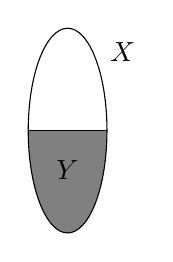
\begin{tikzpicture}
     \begin{scope}
       \clip (0, 0) ellipse (0.5 and 1.3);
        \fill [gray] (-0.5, 0) rectangle (0.5, -1.3);
      \end{scope}
      \draw (0, 0) ellipse (0.5 and 1.3);
      \draw (-0.5, 0) -- (0.5, 0);
      \node at (0, -0.5) {$Y$};
      \node at (0.7, 1) {$X$};
    \end{tikzpicture}
  \end{center}
\end{defi}

\begin{eg}
  For any $x\in X$, the set $I_x = \{y\in x: y< x\}$ is an initial segment. However, not every initial segment of $X$ need to be in this form.

  For example, in $\R$, $\{x: x\leq 3\}$; in $\Q$, $\{x: x < 0\text{ or }x^2 < 2\}$ are both initial segments not of this form.
\end{eg}
However, in a well-ordered, every proper initial segment is of this form.
\begin{prop}
  Every initial segment of a well-ordered set $X$ is of the form $I_x = \{y\in X: y < x\}$.
\end{prop}

\begin{proof}
  Take $x = \min X\setminus Y$. Then $y < x\Rightarrow y\in Y$ by the definition of $x$.  Conversly, if $y\in Y$, then $y < x$ (since $y = x$ and $y > x$ both yield contradictions).
\end{proof}

We want to show that: In a well-ordering $X$, \emph{every} subset $S$ is isomorphic to an initial segment.

\note This is \emph{very} false for a general total order. eg. in $\Z$, take $\{1, 2, 3\}$, but every initial segment of $\Z$ is either infinite or empty. Or, in $\R$, take $\Q$.

It is intuitively obvious that we can do this by sending the minimum element of $S$ to the minimum of $X$, and the continue recursively. However, if we have, say, the double-infinite well-order, then we will never reach the second infinite set. So we need some sort of ``infinite recursion'' that allows us to continue our recursion after infinite time.

We first define the restriction of a function:
\begin{defi}[Restriction of function]
  For $f: A\to B$ and $C\subseteq A$, the \emph{restriction}  of $f$ to $C$ is 
  \[
    f|_C = \{(x, f(x): x\in C\}.
  \]
\end{defi}

\begin{thm}[Definition by recursion]
  Let $X$ be a well-ordered set and $Y$ be any set. Then for any function $G: \P(X\times Y)\to Y$, $\exists f:X\to Y$ such that
  \[
    f(x) = G(F|_{I_x})
  \]
  for all $x$.

  Intuitively, $G$ takes previous values of $f(x)$ and outputs the desired output.

  ``In defining $f$ at $x$, we are allowed to make use of values of $f$ on $I_x$. (eg. $f(x) = nf(n - 1)$ for the factorial function, with $f(0) = 1$)
\end{thm}

\begin{proof}
  We might want to jump into the proof and define $f(0) = G(\emptyset)$, where $0$ is the minimum element, then $f(1) = G(f(0))$ etc., but doing so is simply recursion, which is the thing we want to prove that works!

  Instead, we use the following clever trick: We define an ``$h$ is an attempt'' to mean
  \begin{center}
    $h: I \to Y$, for some initial segment $I$ of $X$, and $h(x) = G(h|_{I_x})$ for $x\in I$.
  \end{center}
  Then we can show that for any $x$, there is an attempt $h$ that is defined at $x$. Then take the value $f(x)$ to be $h(x)$. However, we must show this is well-defined first:

  If attempts $h$ and $h'$ are defined at $x$, then $h(x) = h'(x)$. By induction on $x$, it is enough to show that $h(x) = h'(x)$ assuming $h(y) = h'(y)$ for all $y < x$. But then $h(x) = G(h|_{I_x}) = G(h'|_{I_x}) = h'(x)$.

  Now let's show that for any $x$, there must exist an attempt $h$ that is defined at $x$. Indeed, we may assume (by induction) that for each $y < x$, $\exists$ an attempt $h_y$ defined at $y$. wlog, $h_y$ is defined on all $z \leq y$. Then we put all these functions together, and take $h' = \bigcup_{y < x} h_y$. This is defined for all $y < x$, and is well-defined since the $h_y$ never disagree.

  Finally, add to it $(x, G(h'|_{I_x}))$. Then $h = h'\cup (x, G(h'|_{I_x}))$ is an attempt defined at $x$.

  Now define $f:X\to Y$ by $f(x) = y$ if $\exists$ attempt $h$, defined at $x$, with $h(x) = y$.

  We finally show uniqueness by induction of $x$: suppose $f$ and $f'$ both work. Then if $f(y) = f'(y)$ for all $y < x$, then $f(x) = f'(x)$ by definition. So for all $x$, $f'(x) = f(x)$.
\end{proof}
Now we prove our statement above:
\begin{prop}[Subset collapse]
  Let $X$ be a well-ordering and let $Y\subseteq X$. Then $Y$ is isomorphic to an initial segment of $X$. Moreover, this initial segment is unique.
\end{prop}

\begin{proof}
  For $f: Y\to X$ to be an order-preserving bijection with an initial segment of $X$, we need to map $x$ to the smallest thing not yet mapped to, ie. 
  \[
    f(x) = \min X\setminus \{f(y): y\in Y, y < x\}.
  \]
  (Note: we don't have $\{f(y): y\in Y, y < x\} = X$ because $f(z) \leq z$ for all $z\in Y$ by induction, hence $x$ is not that set)

  Then by the recursion theorem, this function exists and is uniqueness.
\end{proof}
\note So a well-ordered $X$ can \emph{never} be isomorphic to a proper initial segment of $X$, because $X$ is isomorphic to $X$ itself, and uniqueness shows that it cannot be isomorphic to something else.

How do different well-orderings compare?
\begin{notation}
  Write $X\leq Y$ if $X$ is isomorphic to an initial segment of $Y$.
\end{notation}

\begin{eg}
  If $X = \N$, $Y = \{\frac{1}{2}, \frac{2}{3}, \frac{3}{4},\cdots\}\cup \{1\}$, then $X \leq Y$.
\end{eg}

\begin{thm}
  Let $X, Y$ be well-orderings. Then $X\leq Y$ or $Y \leq X$.

  This is ``the best we can hope for''. We cannot find anything analogous for, say, groups.
\end{thm}

\begin{proof}
  Suppose $Y \not\leq X$. For $f: X\to Y$ to be an isomorphism with an initial segment of $Y$, we need $f(x) = \min Y\setminus \{f(y): y < x\}$. We have to make sure that $Y\setminus \{f(y): y < x\}\not= \emptyset$, i.e. $\{f(y): y < x\} \not= Y$. This is true because if we really had $Y = \{f(y): y < x\}$, then we have constructed an isomorphism from $Y$ to an initial segment of $X$.
\end{proof}

\begin{thm}
  Let $X, Y$ be well-orderings with $X\leq Y$ and $Y \leq X$. Then $X$ and $Y$ are isomorphic.
\end{thm}

\begin{proof}
  We have isomorphisms $f: X\to \text{initial segment of }Y$ and $g: Y\to \text{initial segment of }X$. Then $g\circ f: X\to X$ is an isomorphism from $X$ to an initial segment of $X$ (as an initial segment of an initial segment of $X$ is an initial segment of $X$).

  Recall that $X$ is isomorphic to no proper initial segment of $X$. So $g\circ f$ has image $X$. Simiarly, $f\circ g$ is a bijection. So $f$ and $g$ must be bijections.
\end{proof}

\subsection{New well-orderings from old}
We write $X < Y$ if $X\leq Y$ but $X$ is not isomorphic to $Y$, ie. $X$ is isomorphic to a proper initial segment of $Y$.

\subsubsection*{Add one element}
\begin{defi}[Successor]
  Given $X$, choose some $x\not\in X$ and define a well-ordering on $X\cup \{x\}$ by setting $y < x$ for all $y \in X$. This is the \emph{successor} of $X$, written $X^+$.
\end{defi}
Clearly $X < X^+$.
\subsubsection*{Put some together}
\begin{defi}[Extension]
  For well-orderings $(X, <_X)$ and $(Y, <_Y)$, we say $Y$ \emph{extends} $X$ iff $Y > X$, $<_X$ and $<_Y$ agree when defined, and $X$ is an initial segment of $Y$.
\end{defi}

\begin{defi}[Nested family]
  We say well-orderings $(X_i: i\in I)$ form a \emph{nested} family if $\forall i, j\in I$, either $X_i$ extends $X_j$, or $X_j$ extends $X_i$.
\end{defi}

\begin{prop}
  Let $\{X_i: i\in I\}$ be a nested set of well-orderings. Then there exists a well-ordering $X$ with $X\leq X_i$ for all $i$.
\end{prop}
\note This is still true if the $X_i$ are not nested, but the resulting $X$ will not simply be the union of all $X_i$.

\begin{proof}
  Let $X = \bigcup_{i\in I}X_i$ with $<$ defined on $X$ by $< = \bigcup_{i\in I} <_i$ (where $<_i$ is the orderings of $X_i$), i.e. inherit the orders from the $X_i$s. This is a total ordering.

  To see if it is a well-ordering, let $S\subseteq X$ be a non-empty subset of $X$.

  Then $S\cap X_i$ is non-empty for some $i$. Let $x$ be the minimum element (in $X_i$) of $S\cap X_i$. Then also $x \leq y$ for all $y\in S$, as  $X_i$ is an initial segment of $X$.
\end{proof}
This is why we require $X$ to be an initial segment of $Y$ when we define extension. Or else we can take the collection of all subsets $X_n = \{x \geq -n: x\in \Z\}$, and their union would be $\Z$, which is not well-ordered.

\subsection{Ordinals}
Is the collection of all well-orderings (up to isomorphism) itself a well-ordering? We have already shown that it is a total orders.

\begin{defi}[Ordinal]
  An \emph{ordinal} is a well-ordered set, with two regarded as the same if they are isomorphic. We write ordinals as Greek letters $\alpha, \beta$ etc.

  (cf. the rationals consist of all expressions $\frac{m}{n}$, with two regarded as the same if $mn' = nm'$)
\end{defi}
We would want to define ordinals as equivalence classes, but we cannot, because they do not form a set. We will provide a formal treatment later.

\begin{defi}[Order type]
  If a well-ordering $X$ has corresponding ordinal $\alpha$, we say $X$ has \emph{order type} $\alpha$.
\end{defi}

\begin{notation}
  For each $k\in \N$, we write $k$ for the order type of the (unique) well-ordering of size $k$.

  We write $\omega$ for the order type of $\N$.
\end{notation}

\begin{eg}
  In $\R$, $\{2, 3, 5 ,6\}$ has order type 4.

  $\{\frac{1}{2}, \frac{2}{3}, \cdots\}$ has order type $\omega$.
\end{eg}

\begin{notation}
  For ordinals $\alpha, \beta$, write $\alpha \leq \beta$ if $X\leq Y$ for some $X$ of order type $\alpha$, $Y$ of order type $\beta$. This does not depend on the choice of $X$ and $Y$ (since any two choices must be isomorphic).

  We define $\alpha^+$ similarly.
\end{notation}

\begin{prop}
  Let $\alpha$ be an ordinal. Then the ordinals $<\alpha$ form a well-ordering of order type $\alpha$.
\end{prop}

\begin{notation}
  Write $I_\alpha = \{\beta: \beta < \alpha\}$. This is a nice set of order type $\alpha$.
\end{notation}

\begin{proof}
  Let $X$ have order type $\alpha$. The well-orderings $< X$ are precisely (up to isomorphism) the proper initial segments of $X$ (by uniqueness of subset collapse). But these are the $I_x$ for all $x\in X$. These are order-isomorphic to $X$ via $x\mapsto I_x$.
\end{proof}

\begin{prop}
  Let $S$ be a non-empty set of ordinals. Then $S$ has a least element.
\end{prop}

\begin{proof}
  Choose $\alpha\in S$. If it is minimal, done.

  If not, then $S\cap I_\alpha$ is non-empty. But $I_\alpha$ is well-ordered (proposition above). So $S\cap I_\alpha$ has a least element, $\beta$. Then this is a minimal element of $S$
\end{proof}

\begin{thm}[Burali-Forti paradox]
  The ordinals do not form a set.
\end{thm}

\begin{proof}
  Suppose not. Let $X =$ set of ordinals. Then $X$ is a well-ordering. Let its order-type be $\alpha$. Then $X$ is isomorphic to $I_\alpha$, a proper initial subset of $X$. Contradiction
\end{proof}
\note Any set $\{\alpha_i: i\in I\}$ of ordinals has an upper bound ($\alpha$ with $\alpha \geq \alpha_i$ for all $i$). We can apply ``nested well-orders'' to the initial segments $\{I_{\alpha_i}: i\in I\}$. Hence it has a \emph{least} upper bound, $\sup\{\alpha_i: i\in I\}$.

\begin{eg}
  $\{2, 4, 6, 8, \cdots\}$ has supremum $\omega$.
\end{eg}

Now we have two ways of producing ordinals: $+1$ and supremum.

We can generate a lot of ordinals now:

\noindent\begin{tabular}{ccccccc}
  0                                 & $\omega\cdot 2 + 1$             & $\omega^2 + 1$                           & $\omega^2\cdot 3$     & $\omega^{\omega + 2}$                    & $\epsilon_0 + 1$                                 \\
  1                                 & $\omega\cdot 2 + 2$             & $\omega^2 + 2$                           & $\omega^2\cdot 4$     & \vdots                                   & \vdots                                           \\
  2                                 & $\omega\cdot 2 + 3$             & $\omega^2 + 3$                           & $\omega^2\cdot 5$     & $\omega^{\omega \cdot 2}$                & $\epsilon_0 \cdot 2$                             \\
  \vdots                            & \vdots                          & \vdots                                   & \vdots                & \vdots                                   & \vdots                                           \\
  $\omega$                          & $\omega\cdot 3$                 & $\omega^2 + \omega$                      & $\omega^3$            & $\omega^{\omega^2}$                      & $\epsilon_0^2$                                   \\
  $\omega + 1$                      & $\omega\cdot 4$                 & \vdots                                   & \vdots                & \vdots                                   & \vdots                                           \\
  $\omega + 2$                      & $\omega\cdot 5$                 & $\omega^2 + \omega \cdot 2$              & $\omega^\omega$       & $\omega^{\omega^{\omega}}$               & $\epsilon_0^{\epsilon_0}$                        \\
  \vdots                            & \vdots                          & \vdots                                   & \vdots                & \vdots                                   & \vdots                                           \\
  $\omega + \omega = \omega\cdot 2$ & $\omega\cdot \omega = \omega^2$ & $\omega^2 + \omega^2 = \omega^2 \cdot 2$ & $\omega^{\omega + 1}$ & $\omega^{\omega^{.^{.^.}}} = \epsilon_0$ & $\epsilon_0^{\epsilon_0^{.^{.^.}}} = \epsilon_1$ \\
\end{tabular}

Note that officially, $\omega + 1 = \omega^+$, and $\omega \cdot 2= \sup\{\omega, \omega + 1, \omega + 2, \cdots\}$.

All ordinals above are countable, because they are all countable union of countable sets.

Is there an uncountable ordinal? We can well-order $\N$ and $\Q$.

\begin{thm}
  There is an uncountable ordinal.
\end{thm}

\begin{proof}
  We look at the supremum of the set of all countable ordinals. This works only if the collection of countable ordinals is a set.

  Let $A = \{R\in \P(\N\times \N): R \text{ is a well-ordering of a subset of }\N\}$. So $A \subseteq \P(\N\times \N)$. Then $B = \{\text{order type of }R: R\in A\}$ is the set of countable ordinals.
  
  Let $\omega_1 = \sup B$. Then $\omega$ is uncountable. Indeed, if $\omega_1$ is countable, then it is the greatest countable ordinal, but $\omega_1 + 1$ is greater and is also countable.
\end{proof}

\note $\omega_1$ is the \emph{least} uncountable ordinal, by definition, and everything in our previous big list of ordinals is less than $\omega_1$.

There are two strange properties of $\omega_1$:
\begin{enumerate}
  \item $\omega_1$ is an uncountable ordering, yet for every $x\in \omega_1$, the set $\{y: y< x\}$ is countable.
  \item Every sequence in $\omega_1$ is bounded, since its supremum is a countable union of countable sets, which is countable.
\end{enumerate}
In general, we have the following:
\begin{thm}[Hartogs' lemma]
  For any set $X$, there is an ordinal that does not inject into $X$.
\end{thm}

\begin{proof}
  As before, with $B = \{\alpha: \alpha\text{ injects into }X\}$.
\end{proof}

\begin{notation}
  Write $\gamma(X)$ for the least ordinal that does not inject into $X$. eg. $\gamma(\omega) = \omega_1$.
\end{notation}

\subsection{Successors and limits}
Given an ordinal $\alpha$, is there a greatest element of $\alpha$? (ie. does $I_\alpha = \{\beta: \beta < \alpha\}$ have a greatest element?)

If yes, say $\beta$ is the greatest element. Then $\gamma\in I_\alpha \Leftrightarrow \gamma \leq \beta$. So $I_\alpha = \{\beta\}\cup I_\beta$, i.e. $\alpha = \beta^+$.

\begin{defi}[Successor ordinal]
  An ordinal $\alpha$ is a \emph{successor ordinal} if there is a greatest element $\beta$ below it. Then $\alpha = \beta^+$.
\end{defi}

On the other hand, if no, then $\forall \gamma < \alpha, \exists \beta < \alpha$ with $\beta > \gamma$. So $\alpha = \sup \{\beta: \beta < \alpha\}$.
\begin{defi}[Limit ordinal]
  An ordinal $\alpha$ is a limit if it has no greatest element below it. We usually write $\lambda$ for limit ordinals.
\end{defi}

\begin{eg}
  $5$ and $\omega^+$ are successors. $\omega$ and $0$ are limits ($0$ is a limit because it has no element below it, let alone a greatest one!)
\end{eg}

\subsection{Ordinal arithmetic}
We want to define ordinals arithmetic such as $+$ and $\times$, so that we can make formal sense out of our notations $\omega + \omega$ in our huge list of ordinals.

\begin{defi}[Ordinal addition]
  Define $\alpha + \beta$ by recursion on $\beta$ ($\alpha$ is fixed):
  \begin{itemize}
    \item $\alpha + 0 = \alpha$.
    \item $\alpha + \beta^+ = (\alpha + \beta)^+$.
    \item $\alpha + \lambda = \sup \{\alpha + \gamma: \gamma < \lambda\}$ for non-zero limit $\lambda$.
  \end{itemize}
\end{defi}

\begin{eg}
  $\omega + 1 = (\omega + 0)^+ = \omega^+$.

  $\omega + 2 = (\omega + 1)^+ = \omega^{++}$.

  $1 + \omega = \sup\{ 1 + n: n \leq \omega\} \sup\{1, 2, 3, \cdots\} = \omega$.
\end{eg}
So addition is not commutative! This asymmetry arises from our decision to perform recursion on $\beta$ instead of $\alpha$.

\note ``Recursion on the ordinals'' isn't formally allowed because the ordinals do not form a set. Officially, we mean: define $\alpha + \gamma$ on $\{\gamma: \gamma \leq \beta\}$ (which is a set) for each $\beta$. We use the uniqueness of recursion to make sure this is well-defined.

We do this similarly for induction. If $(\forall \beta < \alpha: p(\beta)) \Rightarrow  p(\alpha)$, then if we have $\alpha$ with $p(\alpha)$ false, then $p(\beta)$ is not always true on $\{\beta: \beta \leq \alpha\}$.

\begin{prop}
  Addition is associative, i.e. $(\alpha + \beta) + \gamma = \alpha + (\beta + \gamma)$.
\end{prop}

\begin{proof}
  Since we define addition by recursion, it makes sense to prove this by induction. Since we recursed on the right-hand term in the definition, it only makes sense to induct on $\gamma$ (and fix $\alpha + \beta$).

\begin{enumerate}
  \item If $\gamma = 0$, then $\alpha + (\beta + 0) = \alpha + \beta = (\alpha + \beta) + 0$.
  \item If $\gamma = \delta^+$ is a successor, then 
    \begin{align*}
      \alpha + (\beta + \delta^+) &= \alpha + (\beta + \delta)^+\\
      &= [\alpha + (\beta + \delta)]^+\\
      &= [(\alpha + \beta) + \delta]^+\\
      &= (\alpha + \beta) + \delta^+\\
      &= (\alpha + \beta) + \gamma.
    \end{align*}
  \item If $\gamma$ is a limit ordinal, we have
    \begin{align*}
      (\alpha + \beta) + \lambda &= \sup\{(\alpha + \beta) + \gamma: \gamma < \lambda\}\\
      &= \sup\{\alpha + (\beta + \gamma): \gamma < \lambda\}
    \end{align*}
    If we want to evaluate $\alpha + (\beta + \lambda)$, we have to first know whether $\beta + \lambda$ is a successor or a limit. We now claim it is a limit:

    $\beta + \lambda = \sup\{\beta + \gamma: \gamma < \lambda\}$. This cannot have a greatest element because $\gamma < \gamma' \Rightarrow \beta + \gamma < \beta + \gamma'$, and for each $\beta + \gamma$, we can find a $\gamma' > \gamma$ (because $\lambda$ is a limit) and then $\beta + \gamma' > \beta + \gamma$.

    So
    \[
      \alpha + (\beta + \lambda) = \sup\{\alpha + \delta: \delta < \beta + \lambda\}.
    \]
    We need to show that
    \[
      \sup\{\alpha + \delta: \delta < \beta + \lambda\} = \sup\{\alpha + (\beta + \gamma): \gamma < \lambda\}.
    \]
    Note that the two sets are not equal. For example, if $\beta = 3$ and $\lambda = \omega$, then the left contains $\alpha + 2$ but the right does not.

    So we show that the left is $\geq$ the right and the right is $\geq$ the left.

    $\geq$: Each element of the right hand set is an element of the left.

    $\leq$: For $\delta < \beta + \lambda$, we have $\delta < \sup \{\beta + \gamma: \gamma < \lambda\}$. So $\delta < \beta + \gamma$ for some $\gamma < \lambda$. Hence $\alpha + \delta < \alpha + (\beta + \gamma)$.
\end{enumerate}
\end{proof}
\note  We prove $\beta \leq \gamma \Rightarrow  \alpha + \beta \leq \alpha + \gamma$ by induction on $\gamma$. Hence $\beta < \gamma \Rightarrow  \alpha + \beta < \alpha + \gamma$. But it is not true the other way round: $1 < 2$ but $1 + \omega = 2 + \omega$.

The above definition is called the \emph{inductive} definition. There is also a synthetic definition of $+$.

Intuitively, we first write out all the elements of $\alpha$, then write out all the elements of $\beta$ after it. The $\alpha + \beta$ is the order type of the combined mess.

\begin{defi}[Ordinal addition (synthetic)]
  $\alpha + \beta$ is the order type of $\alpha \sqcup \beta$ ($\alpha$ disjoint union $\beta$, eg. $\alpha\times \{0\}\cup \beta\times \{1\}$), with all $\alpha$ before all of $\beta$
  \[
    \alpha + \beta = \underbracket{\quad\quad\vphantom{\beta}\alpha\vphantom{\beta}\quad\quad}\underbracket{\quad\;\beta\;\quad}
  \]
\end{defi}
\begin{eg}
  $\omega + 1 = \omega^+$.

  $1 + \omega = \omega$.
\end{eg}

With this definition, associativity is trivial:.
\[
  \alpha + (\beta + \gamma) = \underbracket{\quad\quad\vphantom{\beta}\alpha\vphantom{\beta}\quad\quad}\underbracket{\quad\;\beta\;\quad}\underbracket{\quad\gamma\quad} = (\alpha + \beta) + \gamma.
\]
\end{document}
